\documentclass[11pt]{article}
\usepackage{acl-hlt2011}
\usepackage{times}
\usepackage{url}
\usepackage{latexsym}
\usepackage{graphicx}
\usepackage{amsmath}
\usepackage{url}
\usepackage{multirow}
\usepackage{rotating}
%\setlength\titlebox{6.5cm}    
% You can expand the title box if you really have to


\DeclareMathOperator*{\argmax}{arg\,max}

\newcommand{\mnote}[1]{\marginpar{%
  \vskip-\baselineskip
  \raggedright\footnotesize
  \itshape\hrule\smallskip\footnotesize{#1}\par\smallskip\hrule}}  

%\title{Text-to-Text Generation with Syntactic Paraphrases Learned from Bilingual Parallel Corpora}
\title{Learning Sentential Paraphrases from Bilingual Parallel Corpora \\ for Text-to-Text Generation}

\author{Juri Ganitkevitch \and Chris Callison-Burch \and Courtney
  Napoles \and Benjamin Van Durme\\ 
Center for Language and Speech Processing\\ 
Johns Hopkins University}


\author{X\\ 
x\\ 
x\\ 
x}


\date{}

\begin{document}
\maketitle

\begin{abstract}
Previous work has shown that high quality {\it phrasal} paraphrases can be extracted from  bilingual parallel corpora.  However, it is not clear whether bitexts are an appropriate resource for extracting more sophisticated {\it structural} or {\it sentential} paraphrases, which are more obviously learnable from monolingual parallel corpora.
We extend bilingual paraphrase extraction to syntactic paraphrases
and demonstrate its ability to learn variety of general paraphrastic transformations, 
including passivization, dative shift, topicalization, etc.  We discuss how our model can be adapted to many text generation tasks, by augmenting its feature set, development data and parameter estimation routine.  We illustrate this adaptation by using our bilingually extracted paraphrases for the task of sentence compression. 
\end{abstract}


\section{Introduction} \label{introduction}

Paraphrases are alternative ways of expressing the same information. 
Automatically generating and detecting paraphrases is a crucial aspect of many 
natural language processing tasks.
In multi-document summarization, paraphrase detection is used
to collapse redundancies \cite{Barzilay1999,BarzilayThesis}. Paraphrase generation can be used 
for query expansion in information retrieval and question
answering systems \cite{mckeown:1979:ACL,Anick1999,Ravichandran2002,Riezler2007}. 
Paraphrases allow for more flexible matching of system output against human references for tasks like machine translation and automatic summarization \cite{Zhou2006b,Kauchak2006,Owczarzak2006,Madnani2007,Snover2010}. 
%Paraphrases are used to generate additional reference translations for statistical machine translation \cite{Madnani2007} and for more flexible matching when evaluating MT output or automatically generated summaries  \cite{Zhou2006b,Kauchak2006,Owczarzak2006}.

Coarsely, we can distinguish two forms of paraphrases: \emph{phrasal
  paraphrases} denote a set of surface text forms with the same
meaning:
\begin{center}
\begin{tabular}{c}
the committee's second proposal \\
the second proposal of the committee ,
\end{tabular}
\end{center}
while \emph{syntactic paraphrases} augment the surface forms by
introducing nonterminals (or \emph{slots}) that are annotated with
syntactic constraints:
\begin{center}
\begin{tabular}{c}
the $\mathit{NP}_1$'s $\mathit{NP}_2$ \\
the $\mathit{NP}_2$ of the $\mathit{NP}_1$
\end{tabular}
\end{center}
It is evident that the latter have a much higher potential for
generalization and for capturing interesting paraphrastic transformations.

A variety of different types of corpora (and semantic equivalence
cues), have been used to automatically induce paraphrase collections
for English \cite{Madnani2010}. The perhaps most natural type of corpus for this task is
a monolingual parallel text, from which paraphrases can be extracted
by leveraging the fact that the given sentence pairs are perfect
paraphrases of each other \cite{Barzilay2001,Pang2003}. While rich
syntactic paraphrases have been learned from such corpora, they suffer
from very limited data availability and are thus limited by poor
coverage.

Other methods strive to obtain paraphrases from raw monolingual text,
replacing the exact correspondence of sentences in monolingual parallel corpora with
distributional similarity \cite{Lin2001,Bhagat2008}. While
vast amounts of data are readily available for these approaches, the
correspondency information they employ is weaker and suffers from
problems such as mistaking cousin expressions or antonyms (such as
$\{\mathit{boy}, \mathit{girl}\}$ or $\{\mathit{rise},
\mathit{fall}\}$) for paraphrases.

Abundantly available bilingual parallel corpora have been shown to
address both these issues, obtaining paraphrases via a pivoting step
over foreign language phrases \cite{Callison-Burch2005}. The coverage
of paraphrase lexica extracted from bitexts has been shown to
outperform that obtained from other sources \cite{Zhao2008b}. However,
despite existing work on the extraction of more powerful paraphrases
\cite{Madnani2007,Callison-Burch2008,cohn-lapata:2008,Zhao2008}, it is not clear the extent to which sentential paraphrasing can be induced from bitexts. In this paper
we:
\begin{itemize}
\item Extend the bilingual pivoting approach to paraphrase induction
  to produce rich syntactic paraphrases.
\item Perform a thorough analysis of the types of paraphrases we obtain, and discuss the
  paraphrastic transformations we are capable of capturing.
\item Show the resulting paraphrase grammars' fitness and adaptability
  for a variety of text-to-text generation tasks.
\item Describe how training paradigms for
  syntactic/sentential paraphrase models should be tailored to different text-to-text generation tasks. 
\end{itemize}


\section{Related Work} \label{related_work}

\newcite{Madnani2010} survey a variety of data-driven paraphrasing techniques, categorizing them based on the type of data that they use.  \mnote{list the different types of corpora here, and give a laundry list}
%Several research efforts have leveraged parallel monolingual corpora, however they jointly suffer from the scarcity and noisiness of parallel corpora.  \newcite{Dolan2004} work around this issue by extracting parallel sentences from the vast amount of freely available comparable English text and apply machine translation techniques to create a paraphrasing system \cite{Quirk2004}. However, the word-based translation model and monotone decoder they use results in a substantial amount of identity paraphrases or single-word substitutions.


Paraphrase extraction using bilingual parallel corpora was proposed by \newcite{Callison-Burch2005}
who induced paraphrases using techniques from {\it phrase-based}
statistical machine translation \cite{Koehn2003}. After extracting a
bilingual phrase table, English paraphrases can be obtained by
pivoting through foreign language phrases. 
%The phrase table contains
%phrase pairs $(e, f)$ (where the $e$ and $f$ stand for English and
%foreign phrases, respectively) as well as bi-directional 
Since many
paraphrases can be extracted for a phrase, \newcite{Callison-Burch2005} rank them using a paraphrase probability defined in terms of the translation model
probabilities $p(f | e)$ and $p(e | f)$: 

\begin{eqnarray}
  p(e_2|e_1) &=& \sum_f p(e_2,f|e_1)\\
                  &=& \sum_f p(e_2|f,e_1) p(f|e_1) \\
                  &\approx& \sum_f p(e_2|f) p(f|e_1)
\label{paraphrase_prob_eqn}
\end{eqnarray}

Several subsequent efforts extended the bilingual pivoting technique, many of which introduced 
elements of more contemporary {\it syntax-based} approaches to statistical machine translation.   
\newcite{Madnani2007} extended the technique to {\it hierarchical}
phrase-based machine translation \cite{Chiang2005}, which is formally a synchronous context free grammar (SCFG).  Because it is an SCFG,  Madnani's model can be thought of as a {\it  paraphrase grammar}. The paraphrase grammar can paraphrase (or ``decode'') input sentences using an SCFG decoder, like the Hiero, Joshua or cdec MT systems \cite{Chiang2007,Joshua-WMT,Dyer_etal_2010}.
Like Hiero, Madnani's model uses only uses a single nonterminal symbol ``X'' instead of linguistic non-terminals.


Three other papers incorporated linguistic syntax. 
%\newcite{Callison-Burch2008} introduced syntactic constraints by requiring that  paraphrases have the same syntactic type as their phrases.  He did not formally define a synchronous grammar, nor discuss decoding, since his presentation did not include hierarchical rules.
\newcite{Callison-Burch2008} introduced syntactic constraints by labeling all phrases and paraphrases (even non-constituent phrases) with CCG slash categories \cite{Steedman1999}. This is similar  to \newcite{Zollmann2006}'s syntax-augmented machine translation (SAMT). Callison-Burch did not formally define a synchronous grammar, nor discuss decoding, since his presentation did not include hierarchical rules.
\newcite{cohn-lapata:2008} uses the `GHKM' extraction method \cite{Galley2004}, which is limited to constituent phrases and thus produces a reasonably small set of syntactic rules.
\newcite{Zhao2008} added slots to the bilingually-extracted 
paraphrase patterns that were labeled with part-of-speech tags (but not
larger syntactic constituents). 

Before the shift to statistical natural language processing, paraphrasing was often treated as syntactic transformations or by parsing and then generating from a semantic representation \cite{mckeown:1979:ACL,Muraki1982,Meteer1988,Shemtov1996,Yamamoto2002}.  Indeed, some work generated paraphrases used (non-probabilistic) synchronous grammars \cite{Shieber1990,Dras1997,Dras1999,Kozlowski2003}.

After the rise of statistical machine translation, a number of its techniques were re-purposed for paraphrasing.  These include: sentence alignment \cite{Gale1993,Barzilay2003a}, word alignment and noisy channel decoding \cite{Brown1990,Quirk2004}, phrase-based models \cite{Koehn2003,Callison-Burch2005}, hierarchical phrase-based models \cite{Chiang2005,Madnani2007}, log linear models and minimum error rate training \cite{Och2003c,Madnani2007,Zhao2008b}, and here syntax-based machine translation \cite{Wu1997,Yamada2001,Melamed2004,Quirk2005}.


Beyond cementing the ties between paraphrasing and syntactic-based statistical machine translation, the novel contributions of our paper are (1) an in-depth analysis of the types of structural and sentential paraphrases that can be extracted with bilingual pivoting, (2) instructions on how our English-English paraphrase grammar should be adapted to specific text to text generation tasks \cite{zhao-EtAl:2009:ACLIJCNLP2} with (3) a concrete example of the adaptation procedure for the task of paraphrase-based sentence compression \cite{KnightMarcuAI02,cohn-lapata:2008,Cohn2009}.



%Relying on small data sets of semantically equivalent translations, \newcite{Pang2003} created finite state automata by syntax-aligning parallel sentences, enabling the generation of additional reference translations.

%Both \newcite{Barzilay2001} and \newcite{Ibrahim2003} sentence-align existing noisy parallel monolingual corpora such as translations of the same novels. While \newcite{Ibrahim2003} employ a set of heuristics that rely on anchor words identified by textual identity or matchin liguistic features such as gender, number or semantic class, \newcite{Barzilay2001} use a co-training approach that leverages context similarity to identify viable paraphrases.

%Semantic parallelism is well-established as a stong basis for the extraction of correspondencies such as paraphrases. However, there are notable efforts that choose to forgo it in favor of clustering approaches based on distributional characteristics. The well-known DIRT method by \newcite{Lin2001} fully relies on distributional similarity features for paraphrase extraction. Patterns extracted from paths in dependency graphs are clustered based on the similarity of the observed contents of their slots.

%Similarly, \newcite{Bhagat2008} argue that vast amounts of text can be leveraged to make up for the relative weakness of distributional features compared to parallelism. They also forgo complex annotations such as syntactic or dependency parses, relying only on part-of-speech tags to inform their approach. In their work, relations are learned by finding pattern clusters initially seeded by already known patterns. However, this method is not capable of producing syntactic paraphrases. \mnote{Need better tie-in with the overall theme of  structural paraphrases.}


\section{SCFGs in Translation} \label{formalism}

The model we use in our paraphrasing approach is a syntactically
informed \emph{ synchronous context-free grammar} (SCFG).  The SCFG formalism \cite{Aho1972}  was re-popularized for statistical machine translation by \newcite{Chiang2005}.  
Formally, a \emph{probabilistic} SCFG $\mathcal{G}$ is defined by
specifying
\[
\mathcal{G} = \langle \mathcal{N}, \mathcal{T}_S, \mathcal{T}_T,
\mathcal{R}, S \rangle ,
\]
where $\mathcal{N}$ is a set of nonterminal symbols, $\mathcal{T}_S$
and $\mathcal{T}_T$ are the source and target language vocabularies,
$\mathcal{R}$ is a set of rules and $S \in \mathcal{N}$ is the root
symbol. The rules in $\mathcal{R}$ take the form
\begin{equation*}
  C \rightarrow \langle \gamma, \alpha, \sim, w \rangle ,
\end{equation*}
where the rule's left-hand side $C \in \mathcal{N}$ is a nonterminal,
$\gamma \in (\mathcal{N} \cup \mathcal{T}_S)^*$ and $\alpha \in
(\mathcal{N} \cup \mathcal{T}_T)^*$ are strings of terminal and
nonterminal symbols with an equal number of nonterminals
$c_{\mathit{NT}}(\gamma) = c_{\mathit{NT}}(\alpha)$ and 
$$
\sim : \{1 \ldots c_{\mathit{NT}}(\gamma)\} \rightarrow \{1 \ldots
c_{\mathit{NT}}(\alpha)\}
$$ 
constitutes a one-to-one correspondency function between the
nonterminals in $\gamma$ and $\alpha$. A non-negative weight $w \geq
0$ is assigned to each rule, reflecting the likelihood of the rule.


\begin{figure}[t]
\begin{center}
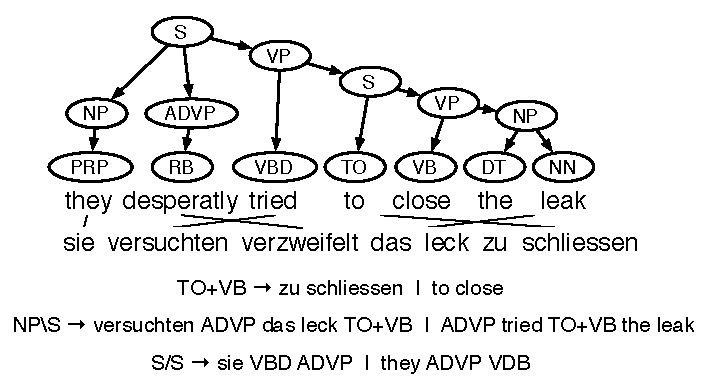
\includegraphics[width=0.99\linewidth]{figures/example_extraction.pdf}
\end{center}
\caption{TODO: write caption}
\label{example_extraction}
\end{figure}

%\paragraph{Extracting rules from bitexts}
\paragraph{Rule Extraction}

Phrase-based approaches to statistical machine translation (and their successors) extract pairs of $(e, f)$ phrases from automatically word-aligned parallel sentences. \newcite{Och2003}
%, \newcite{Koehn2004}, \newcite{Tillmann2003}, and \newcite{Vogel2003} 
described various heuristics for extracting phrase alignments from the Viterbi word-level alignments that are estimated using \newcite{Brown1993} word-alignment models.  

These phrase extraction heuristics have been extended so that they extract synchronous grammar rules \cite{Galley2004,Chiang2005,Zollmann2006,Liu2006}.  Most of these extraction methods require that one side of the parallel corpus be parsed, typically this is done automatically with a statistical parser.  

\mnote{ccb - todo - tighten this up.}   
  The rule set
for our synchronous grammar is extracted from word-aligned
sentence-parallel corpora where the target language side is annotated
with syntactic parses. Figure~\ref{example_extraction} shows examples
of rules obtained from a sentence pair. To extract a rule, we first
choose a target span $e$. The left-hand side of the rule is then given
by the syntactic constituent governing $e$. However, in doing so we
can only assign left-hand side labels to a small portion of the
possible phrases in a sentence pair. To allow for broader coverage, we
rely on the labeling method introduced by \newcite{Zollmann2006}: in
addition to single constituent nonterminals, we allow for the
concatenation of constituents as well as for CCG-style slashed
constituents \cite{Steedman1999}.

The source side of the rule, $f$, is obtained by projecting $e$ over
the word alignment. To introduce nonterminals into the rule body, we
can apply rules extracted over sub-phrases of $e$, synchronously
substituting the corresponding nonterminal symbol for the sub-phrases
on both sides. The synchronous substitution applied to $e$ and $f$
then yields the correspondency $\sim$.


\paragraph{Feature functions}

Rather than assigning a single weight $w$, we define a number of feature
functions $\varphi_i$, which are combined in a log-linear model:
\begin{equation}
  w = \sum_i^N \lambda_i \varphi_i .
\end{equation}
For ease of notation, we will refer to $\varphi_1, \ldots ,\varphi_N$
as $\vec{\varphi}$. 
The weights $\vec{\lambda}$ of the these feature functions are set to maximize some objective function like Bleu \cite{Papineni2002} using a procedure called minimum error rate training \cite{Och2003c}.  MERT iteratively adjusts the weights until the decoder produces output that best matches reference translations in a development set, according to the objective function.  We will examine appropriate objective functions for text-to-text generation tasks in Section \ref{dev-data-and-objective-functions}.

Typical features used in statistical machine translation include:\mnote{TODO: Juri list out typical feature functions  -- they can be less formal than this}
\begin{itemize}
\item The feature set of the translation model by
default consists of the negative lexical translation log-probabilities
\[
\varphi_{\mathit{lex}} = \langle -\log p_{\mathit{lex}}(e | f), -\log
p_{\mathit{lex}}(f | e)\rangle
\]
and its phrasal counterpart $\varphi_{\mathit{phrase}}$. 

\item Count features $c_{\mathit{src}}$ and $c_{\mathit{tgt}}$
  indicating the number of words on either side of the rule as well as
  two difference features, $c_{\mathit{dcount}} = c_{\mathit{tgt}} -
  c_{\mathit{src}}$ and the analoguosly computed difference in the
  average word length in characters, $c_{\mathit{davg}}$.

\item An incidator for when a rule only contains terminal symbols
  ($\delta_{\mathit{lex}}$) and an indicator for when the source side
  contains terminals, but the target side does not
  ($\delta_{\mathit{del}}$).

%\item Indicators for whether the rule swaps the order of two
%  nonterminals ($\delta_{\mathit{reorder}}$) and whether the two
%  nonterminals are adjacent ($\delta_{\mathit{adj}}$).

\item A rarity penalty $\varphi_{\mathit{rarity}} =
  e^{(1-c_{\mathit{rule}})}$ that quantifies the doubt we may place in
  a rule based on how often we have encountered it in the
  corpus\footnote{Since we do not have an immediate rule count for a
    paraphrase rule $N \rightarrow e_1 | e_2$, we instead estimate
    its rarity penalty as $\varphi_{\mathit{rarity}}(N
    \rightarrow e_1 | e_2) = \max_{f} \min
    \{\varphi_{\mathit{rarity}}(N \rightarrow e_1 | f),
    \varphi_{\mathit{rarity}}(N \rightarrow f | e_2) \}$}.
\end{itemize}








\paragraph{Decoding}

Given an SCFG and an input source sentence, the decoder performs the search for the single most probable or $k$-best translations using the CKY algorithm. 

\begin{figure}[t]
\begin{center}
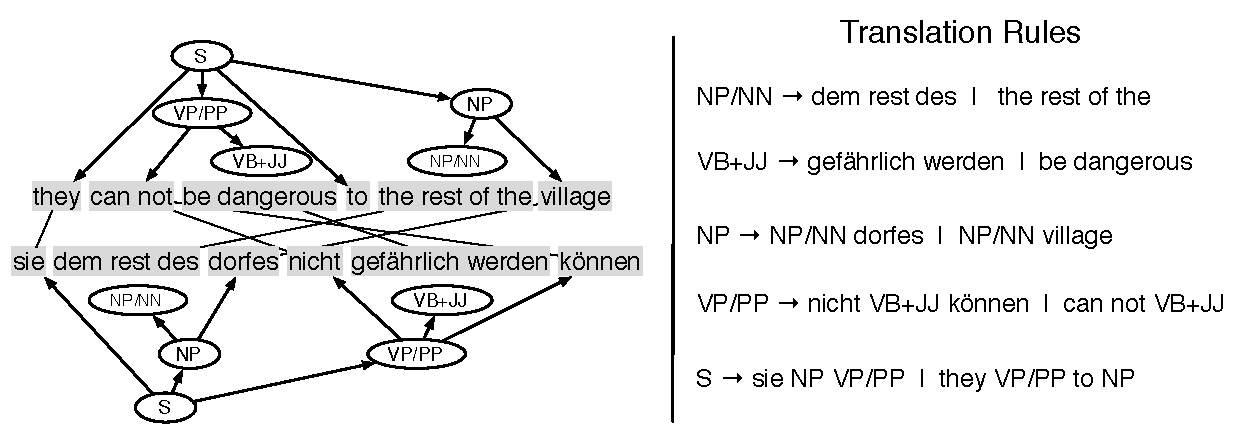
\includegraphics[width=0.99\linewidth]{figures/example_translation.pdf}
\end{center}
\caption{An example derivation produced by a syntactic machine translation system.  Although the synchronous trees are unlike the derivations found in the Penn Treebank, their yield is a good translation of the German.}
\label{example_translation}
\end{figure}


\section{SCFGs in Paraphrasing} \label{acquisition}

\begin{figure}[!t]
\begin{center}
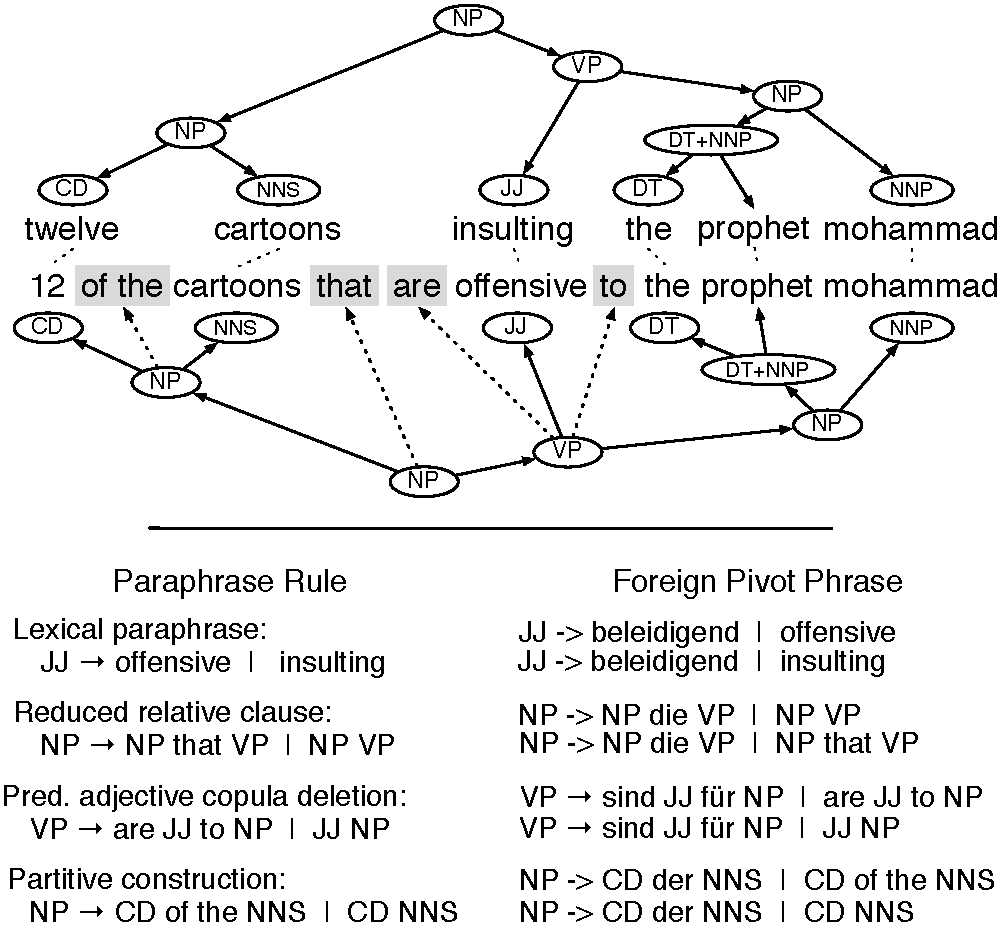
\includegraphics[width=0.99\linewidth]{figures/example_compression_1col.pdf}
\end{center}
\caption{An example of a synchronous paraphrastic derivation. A few of
  the rules applied in the parse are show in the second column, with
  the pivot phrases that gave rise to them in the third.}
\end{figure}

To create a paraphrase grammar from a translation grammar, we extend
the syntactically informed pivot approach of
\newcite{Callison-Burch2008} to the SCFG model. For this purpose, we
assume a grammar that translates from a given foreign language to
English. For each pair of translation rules where the left-hand side
$C$ and foreign string $\gamma$ match
\begin{eqnarray*}
C \rightarrow \langle \gamma, \alpha_1, \sim_1, \vec{\varphi}_1 \rangle \\
C \rightarrow \langle \gamma, \alpha_2, \sim_2, \vec{\varphi}_2 \rangle
\end{eqnarray*}
we create a paraphrase rule
\begin{equation*}
C \rightarrow \langle \alpha_1, \alpha_2, \sim, \vec{\varphi} \rangle ,
\end{equation*}
where the nonterminal correspondency relation $\sim$ has been set to
reflect the combined nonterminal alignment
\begin{equation*}
\sim ~ = ~ \sim_1^{-1} \circ \sim_2 .
\end{equation*}

In the computation of the features $\vec{\varphi}$ from
$\vec{\varphi}_1$ and $\vec{\varphi}_2$ we follow the approximation in
Equation~\ref{paraphrase_prob_eqn}, which yields lexical and phrasal
paraphrase probability features.


\begin{itemize}
\item A boolean indicator for whether the rule is an identity
  paraphrase, $\delta_{\mathit{identity}}$.
  \item Indicators for whether the rule swaps the order of two
  nonterminals ($\delta_{\mathit{reorder}}$) 
\end{itemize}

The other advantage of using the decoder from statistical machine translation is that n-gram language models, which have been shown to be useful in natural language generation \cite{Langkilde1998}, are already well integrated \cite{Liang-and-david}.



%\subsection{Grammar Pruning}\label{pruning}

%Due to the diverse set of nonterminals allowed in our model, the grammars we extract tend to become extremely large. This, combined with the multiplicative effect of pivoting, quickly makes the resulting paraphrase grammars grow too large too handle.

%To keep the grammars at a manageable size while retaining good paraphrases, we implement the following pruning approach. We only consider translation rules that have been seen more than $c_{\mathit{min}}$ times and exceed a given translation probability threshold $p_{\mathit{min}}$ for pivot recombination. In addition to this, we rank the generated paraphrases for each foreign pivot phrase according to a uniformly weighted combination of phrasal and lexical paraphrase probabilities and only retain the top $n$ most likely alternatives.

%The result of this process is a paraphrase grammar with syntactic annotations and a feature set which (approximately) mirrors that of the initial translation grammar.


\section{Analysis} \label{analysis}

\begin{table*}[!ht]
  \begin{center}
  \begin{tabular}{|c|rrcl|}
    \hline
    \multirow{2}{*}{Possessive rule} & $\mathit{NP}$ $\rightarrow$ & the
    $\mathit{NN}$ of the $\mathit{NNP}$ & $\mid$ & the
    $\mathit{NNP}$'s $\mathit{NN}$ \\
    & $\mathit{NP}$ $\rightarrow$  & the $\mathit{NNS}_1$ made by
    $\mathit{NNS}_2$ & $\mid$ & the $\mathit{NNS}_2$'s
    $\mathit{NNS}_1$ \\
    \hline
    \multirow{2}{*}{Dative shift} & $\mathit{VP}$ $\rightarrow$ & give
    $\mathit{NN}$ to $\mathit{NP}$ & $\mid$ & give $\mathit{NP}$ the
    $\mathit{NN}$ \\
    & $\mathit{VP}$ $\rightarrow$ & provide $\mathit{NP}_1$ to
    $\mathit{NP}_2$ & $\mid$ & give $\mathit{NP}_2$
    $\mathit{NP}_1$ \\
    \hline
    \hline
    \multirow{2}{*}{Adv./adj. phrase move} & 
    $\mathit{S/VP}$ $\rightarrow$ & $\mathit{ADVP}$ they $\mathit{VBP}$
    & $\mid$ & they $\mathit{VPB}$ $\mathit{ADVP}$ \\
    & $\mathit{S}$ $\rightarrow$ & it is $\mathit{ADJP}$ $\mathit{VP}$
    & $\mid$ & $\mathit{VP}$ is $\mathit{ADJP}$ \\
    \hline
    Verb particle shift & 
    $\mathit{VP}$ $\rightarrow$ & $\mathit{VB}$ $\mathit{NP}$ up &
    $\mid$ & $\mathit{VB}$ up $\mathit{NP}$ \\
    \hline
    \multirow{2}{*}{Reduced relative clause} & $\mathit{SBAR/S}$ $\rightarrow$ &
    although $\mathit{PRP}$ $\mathit{VBP}$ that & $\mid$ &although
    $\mathit{PRP}$ $\mathit{VBP}$ \\
    & $\mathit{ADJP}$ $\rightarrow$ &
    very $\mathit{JJ}$ that $\mathit{S}$ & $\mid$ & $\mathit{JJ}$ $\mathit{S}$ \\
    \hline
    \multirow{2}{*}{Quantificational variants} & 
    $\mathit{NP}$ $\rightarrow$ & $\mathit{CD}$ of the $\mathit{NN}$
    & $\mid$ & $\mathit{CD}$ $\mathit{NN}$ \\
    & $\mathit{NP}$ $\rightarrow$ & all $\mathit{DT\backslash NP}$
    & $\mid$ & all of the $\mathit{DT\backslash NP}$ \\
    \hline
    Topicalization  & $\mathit{S}$ $\rightarrow$ & $\mathit{NP}$,
    $\mathit{VP}$ . & $\mid$ & $\mathit{VP}$, $\mathit{NP}$ . \\
    \hline
    \hline
    Passivization &
    $\mathit{SBAR}$ $\rightarrow$ & that $\mathit{NP}$ had
    $\mathit{VBN}$ & $\mid$ & which was $\mathit{VBN}$ by $\mathit{NP}$ \\
    \hline
    \multirow{2}{*}{Light verbs} & $\mathit{VP}$ $\rightarrow$ & take action $\mathit{ADVP}$ &
    $\mid$ & to act $\mathit{ADVP}$ \\
    & $\mathit{VP}$ $\rightarrow$ & $\mathit{TO}$ take a decision $\mathit{PP}$ &
    $\mid$ & $\mathit{TO}$ decide $\mathit{PP}$ \\
    \hline
\end{tabular}
\end{center}
\caption{Examples of meaning-preserving transformations and syntactic
  paraphrases that our system extracts to capture them.}
\label{example_rules}
\end{table*}


A key motivation for the use of syntactic paraphrases over their
phrasal counterparts is their potential to capture meaning-preserving
linguistic transformations in a general fashion. In many cases a
phrasal system will be limited to memorizing the fully lexicalized
variants of such a transfomation in its paraphrase table, resulting in
poor generalization capabilities. A syntactic paraphrasing system
should be able to address this issue by learning syntactically
well-formed and generic patterns that can be easily applied to unseen
data.

To put this expectation to the test, we investigate how our grammar
captures a number of well-known paraphrastic
transformations.\footnote{For this analysis, we extracted a paraphrase grammar from the French-English Europarl corpus (v5). The bitext was aligned using the Berkeley aligner and the English side was parsed using the Berkeley parser. We obtained the initial translation grammar using the SAMT toolkit. }
Table~\ref{example_rules} shows the transformations
along with examples of the generic grammar rules our system learns to
represent them. When given a transformation to extract a syntactic
paraphrase for, we want to find rules that neither under- nor
over-generalize. This means that, while replacing the maximum number
of \emph{syntactic} arguments with nonterminals, the rules ideally
will both retain enough lexicalization to serve as sufficient evidence
for the applicability of the transformation and impose constraints on
the nonterminals to ensure the arguments' well-formedness.

The paraphrases implementing the \emph{possessive rule} and the
\emph{dative shift} shown in Table~\ref{example_rules} are a good
examples of this: the two noun-phrase arguments to the expressions are
abstracted to nonterminals while the rules' lexicalization provides an
appropriate frame of evidence for the transform. This is important for
a good representation of the dative shift, which is a reordering
transformation that fully applies to certain di-transitive verbs while
other verbs are uncommon in one of the forms:
\begin{center}
\begin{tabular}{l}
  give \emph{decontamination equipment} to \emph{Japan} \\
  give \emph{Japan} \emph{decontamination equipment} \\
  \vspace{-10pt}\\
  provide \emph{decontamination equipment} to \emph{Japan} \\
  ? provide \emph{Japan} \emph{decontamination equipment} \\
\end{tabular}
\end{center}
Note how our system extracts a dative shift rule for \emph{to give}
and a rule that both shifts and substitutes a more appropriate verb
when paraphrasing \emph{to provide}.

\newcite{Madnani2007} generalize from phrasal paraphrases with the
Hiero formalism, which uses SCFG rules with a single nonterminal
$X$. We use syntactic nonterminals in our paraphrase rules to capture
complex transforms that also impose appropriate constraints on their
application. Since \newcite{Madnani2007} do not impose any constraints
on how the nonterminal $X$ can be realized, their equivalent of the
\emph{topicalization} rule
\mnote{I think that our version of the topicalization rule should be $\mathit{S}$ $\rightarrow$  $\mathit{S/NP}$ $\mathit{NP}$.  $\mid$ $\mathit{NP}$, $\mathit{S/NP}$.  I.e. \emph{I like these bagels!  $\mid$ These bagels, I like!}   }
\begin{center}
\begin{tabular}{rrcl}
  $\mathit{S}$ $\rightarrow$ & $\mathit{X}_1$,
  $\mathit{X}_2$ . & $\mid$ & $\mathit{X}_2$, $\mathit{X}_1$ . \\
\end{tabular}
\end{center}
would massively overgeneralize. Additional examples of transforms our
use of syntax allows us to capture are the \emph{adverbial phrase 
 shift} and the \emph{reduction of a relative clause}.
 
Unsurprisingly, syntactic information alone is not sufficient to
capture all transformations. For instance it is hard to extract
generic paraphrases for all instances of \emph{passivization}, since our syntactic
model currently has no means of representing the morphological changes that the
verb undergoes:
\begin{center}
\begin{tabular}{l}
%  the cat \emph{ate} the mouse \\
%  the mouse \emph{was eaten} by the cat \\
  the reactor \emph{leaks} radiation \\
  radiation \emph{is leaking} from the reactor\\
\end{tabular}

\end{center}
Still, for cases where verb's morphology does not change, we manage to
learn a rule:
\begin{center}
\begin{tabular}{l}
%  the mouse that the cat had \emph{eaten} \\
%  the mouse which was \emph{eaten} by the cat \\
the radiation that the reactor had \emph{leaked} \\
the radiation which \emph{leaked} from the reactor \\
\end{tabular}
\end{center}
%
Another example of a deficiency in our synchronous grammar models are
\emph{light verb} constructs such as
\begin{center}
\begin{tabular}{l}
  to take a \emph{walk} \\
  to \emph{walk} .
\end{tabular}
\end{center}
Here, a noun is transformed into the corresponding verb -- something
our synchronous syntactic CFG approach is not able to capture except
through memorization.

Overall our survey shows that we are able to extract appropriately generic
representations for a surprising number of paraphrastic
transformations, far exceeding the expressiveness of previous
approaches to paraphrase extraction from bilingual parallel corpora.



% \subsection{Comparison of Paraphrase
%   Patterns} \label{pattern_comparison}

% To analyze the paraphrase patterns produced by our system, we reduce
% the grammar to only patterns that apply to an example sentence and
% take a closer look at the most likely pattern pairs. We contrast our
% extracted paraphrases with a Hiero-style baseline that mirrors the
% approach of \newcite{Madnani2007}. 

% \begin{table*}[t]
% \begin{center}
% \begin{tabular}{|c|c|rrcl|}
%   \hline
%   Input phrase & \multicolumn{5}{c|}{Best extracted paraphrases} \\
%   \hline
%   \multirow{6}{*}{the dog's tail} &
%   \multirow{3}{*}{H}
%   &
%   $\mathit{X}$ $\rightarrow$  & the $\mathit{X}_1$'s
%   $\mathit{X}_2$ & $\mid$ & the $\mathit{X}_2$ of the $\mathit{X}_1$
%   \\
%   &&
%   $\mathit{X}$ $\rightarrow$  & the $\mathit{X}_1$'s
%   $\mathit{X}_2$ & $\mid$ & the $\mathit{X}_2$ of the $\mathit{X}_1$
%   \\
%   &&
%   $\mathit{X}$ $\rightarrow$  & the $\mathit{X}_1$'s
%   $\mathit{X}_2$ & $\mid$ & the $\mathit{X}_2$ of the $\mathit{X}_1$ \\
%   \cline{2-6}
%   & \multirow{3}{*}{S}
%   &
%   $\mathit{NP}$ $\rightarrow$  & the $\mathit{NNP}_1$'s
%   $\mathit{NN}_2$ & $\mid$ & the $\mathit{NN}_2$ of the $\mathit{NNP}_1$
%   \\
%   &&
%   $\mathit{NP}$ $\rightarrow$  & the $\mathit{NNP}_1$'s
%   $\mathit{NN}_2$ & $\mid$ & the $\mathit{NN}_2$ of the $\mathit{NNP}_1$
%   \\
%   &&
%   $\mathit{NP}$ $\rightarrow$  & the $\mathit{NNP}_1$'s
%   $\mathit{NN}_2$ & $\mid$ & the $\mathit{NN}_2$ of the
%   $\mathit{NNP}_1$ \\
%   \hline
%   \multirow{6}{*}{the dog's tail} &
%   \multirow{3}{*}{H}
%   &
%   $\mathit{X}$ $\rightarrow$  & the $\mathit{X}_1$'s
%   $\mathit{X}_2$ & $\mid$ & the $\mathit{X}_2$ of the $\mathit{X}_1$
%   \\
%   &&
%   $\mathit{X}$ $\rightarrow$  & the $\mathit{X}_1$'s
%   $\mathit{X}_2$ & $\mid$ & the $\mathit{X}_2$ of the $\mathit{X}_1$  \\
%   &&
%   $\mathit{X}$ $\rightarrow$  & the $\mathit{X}_1$'s
%   $\mathit{X}_2$ & $\mid$ & the $\mathit{X}_2$ of the $\mathit{X}_1$
%   \\
%   \cline{2-6}
%   & \multirow{3}{*}{S}
%   &
%   $\mathit{NP}$ $\rightarrow$  & the $\mathit{NNP}_1$'s
%   $\mathit{NN}_2$ & $\mid$ & the $\mathit{NN}_2$ of the $\mathit{NNP}_1$
%   \\
%   &&
%   $\mathit{NP}$ $\rightarrow$  & the $\mathit{NNP}_1$'s
%   $\mathit{NN}_2$ & $\mid$ & the $\mathit{NN}_2$ of the $\mathit{NNP}_1$
%   \\
%   &&
%   $\mathit{NP}$ $\rightarrow$  & the $\mathit{NNP}_1$'s
%   $\mathit{NN}_2$ & $\mid$ & the $\mathit{NN}_2$ of the
%   $\mathit{NNP}_1$ \\
%   \hline
% \end{tabular}
% \end{center}
% \caption{This table shows the top paraphrase rules matching an input
%   phrase as ranked by our (S) and the baseline system (H).}
% \end{table*}


\section{Text-to-Text Applications} \label{adaptation}

The core of many text-to-text generation tasks is sentential
paraphrasing, augmented with specific constraints or goals. Since in
our model we are borrowing much of the machinery from statistical
machine translation -- a sentential rewriting problem itself -- it is
straightforward to use our paraphrase grammars to generate new
sentences using its decoding and parameter optimization
techniques. The SMT framework can be adapted to many different
text-to-text generation tasks.  These could include text
simplification, sentence compression, poetry generation, query
expansion, transforming declarative sentences into questions, deriving
hypotheses for textual entailment, etc.  Each individual text-to-text
application requires that the SMT framework be adapted in several
ways, by specifying:
\begin{itemize}
\item A mechanism for extracting synchronous grammar rules (in this
  paper we argue that pivot-based paraphrasing is widely applicable)
\item An appropriate set of rule-level features that capture pertinent
  information about the task (i.e.\ whether a rule simplifies a
  phrase)
\item An appropriate `objective function' that scores the output of
  the model.  This is a task-specific equivalent to the Bleu metric in
  SMT.
\item A development set with examples of the sentential
  transformations that we are modeling.
  % The dev set is used with the objective function to set the weights
  % of the features.
\item Optionally, a way of injecting task-specific rules that were not
  extracted automatically.
\end{itemize} 
In the remainder of this section, we illustrate how our bilingually
extracted paraphrases can be adapted to perform sentence compression,
which is the task of reducing the length of sentence while preserving
its core meaning.  Most previous approaches to sentence compression
focused only on the deletion of a subset of words from the sentence
\cite{KnightMarcuAI02}.  Our approach follows
\newcite{cohn-lapata:2008}, who expand the task to include
substitutions, insertions and reorderings that are automatically
learned from parallel texts.

\subsection{Feature Design}
In Section~\ref{acquisition} we discussed the phrasal and lexical
paraphrasing features $\varphi_{\mathit{lex}}$ and
$\varphi_{\mathit{phrase}}$. While these features quantify the quality
of a paraphrase, they do not make any statement on the change in
language complexity or text length, nor do they bear any information
on the degree and nature of the transformation that the rule
effects. To make this infromation available to the decoder, we enhance
our paraphrases with the following features:
\begin{itemize}
\item Count features $c_{\mathit{src}}$ and $c_{\mathit{tgt}}$
  indicating the number of words on either side of the rule as well as
  two difference features, $c_{\mathit{dcount}} = c_{\mathit{tgt}} -
  c_{\mathit{src}}$ and the analoguosly computed difference in the
  average word length in characters, $c_{\mathit{davg}}$.
\end{itemize}


\subsection{Development Data and Objective Function}
\label{dev-data-and-objective-functions}
To tune the parameters of our paraphrase system to perform sentence
compression, we have created a corpus of compression
paraphrases. Beginning with 9570 tuples of parallel English sentences
obtained from translation references for various machine translation
tasks, we obtained a parallel compression corpus by selecting the
longest reference in each tuple as the source sentence and the
shortest reference as the target sentence and retaining only those
sentence pairs where the word count ratio $r$ was $0.5 < r \leq
0.8$. From these, we then randomly selected 936 sentences for the
development set, as well as 815 sentences for a test set that we later
use to gauge the performance of our system.

Due to the compressive nature of the resulting corpus, we deemed the
widely used BLEU metric \cite{Papineni2002} to be sufficient to judge
the system's compression performance in parameter estimation.

As our method of parameter estimation, we chose minimum error rate
training \cite{Och2003c} using the Z-MERT and the Joshua toolkits
\cite{Zaidan2009,Joshua-WMT}.



\subsection{Grammar Injections} \label{injection}

As we discussed in Section~\ref{analysis}, the paraphrase grammar we
induce is capable of representing a wide variety of
transformations. However, the formalism and extraction method are not
explicitely geared towards a compression application. For instance,
the synchronous nature of our grammar does not allow us to perform
deletions of constituents as done by \newcite{Cohn2007}.  A possible
way to extend the grammar's capabilities towards the requirements of a
given task is by injecting additional rules designed to capture
appropriate operations. 

For the compression task, this can include adding rules that allow
generic deletions of target-side nonterminals\footnote{This renders
  the SCFG asynchronous and requires appropriate adjustments in the
  decoding process.}, or generating rules that specifically delete
particular adjectives from the corpus\footnote{Note that since we do
  not learn these rules from data, we cannot estimate their cost from
  translation probabilities or counts. In a discriminative setting
  each rule will correspond to a feature. We leave the investigation
  of this to future work. TODO.}:
\begin{center}
\begin{tabular}{cc}
 $\mathit{JJ} \rightarrow$ & $\mathit{JJ} \mid \varepsilon$ \\
 $\mathit{JJ} \rightarrow$ & superfluous $\mid \varepsilon$ . \\
\end{tabular}
\end{center}
In our system, we implemented the injection of rules that improve the
handling of out-of-vocabulary words. Typically an SMT system will
generate heavily penalized identity translation rules for all words in
an input sentence, to assure that the OOV rules will only apply when
there is no translation rule for a particular word. For our
paraphrasing approach however, encountering an unknown word is not
critical as long as we can assign it the proper syntactic label. To
enable our system to process unseen words in the input, we allow for
syntactically parsed input and for every input word $w$ include rules
of the form $\mathit{T} \rightarrow w \mid w$, where $T$ is the
part-of-speech tag assigned to $w$ in the input parse. To enable a
proper inclusion into the paraphrasing model, we add a constant
penalty feature $\varphi_{\mathit{oov}}$ and include its weight in our
parameter estimation process.

\subsection{Evaluation} \label{evaluation}

To assess our sentence compression system's performance we perform a
human evaluation on Amazon Mechanical Turk, comparing it to both an
unadapted paraphrase grammar and an implementation of the ILP-based
sentence compression system introduced by \newcite{Clarke2008}.

Our method achieves relatively low compression rates (when compared to
deletion-centric compression approaches such as \newcite{Clarke2008}
or \newcite{Cohn2007}). This can be explained by our system being a
compressive paraphraser rather than an aggressively deletion-orieneted
model: the model achieves compression by removing syntactic
redundancies and replacing legthily worded expressions by shorter
ones. It does not intentionally perform neither word- nor
constituent-level deletions and is therefore naturally limited in the
achievable compression rate. Since the quality of a compression (as
judged by humans) strongly correlates with the compression rate, we
constrain the ILP implementation to achieve the same compression rate
for each sentence as our system.

We collect human judgments on the quality of the compressions on
MTurk. TODO: expand this with the details.

The results are shown in Table~\ref{human_judgments}. We can see that
some systems do better than others, hopefully systematically so. With
any luck, we even manage to hold our ground to the ILP
implementation. Oh wonder, oh joy. TODO.

\begin{table}
\begin{center}
\begin{tabular}{|c|c|c|}
  \hline
  System & Compression & Score \\
  \hline
  Hiero & ?? & ?? \\
  Syntax & ?? & ?? \\
  Syntax + Features & ?? & ?? \\
  ILP & ?? & ?? \\
  \hline
\end{tabular}
\end{center}
\caption{TODO: obtain proper scores}
\label{human_judgments}
\end{table}



\section{Conclusion} \label{conclusion}

In this work we introduced a method to learn syntactically informed
paraphrases from bilingual parallel texts. We discuss the expressive
power and limitations of our formalism and demonstrate its
applicability to text-to-text generation on the example of sentence
compression.

% \section*{Acknowledgments}
% We would like to thank Trevor Cohn for kindly providing us with
% access to data sets and the T3 compression system and Ben Van Durme
% for helpful discussions.

\bibliographystyle{acl}
\bibliography{paraphrasing}


\end{document}

